\section{Transaktionen}
\begin{displayquote}
    "Eine Folge von Datenbankanweisungen, welche entweder ganz oder garnicht ausgeführt wird."
\end{displayquote}
\subsection{Allgemeines}
\subsubsection{ACID Prinzip}
\begin{itemize}
    \item Atomicity $\implies$ Transaktion ist die kleinste Arbeitseinheit, sie wird entweder ganz oder garnicht ausgeführt
    \item Consistency $\implies$ Die Datenbank ist zu Beginn und Ende jeder Transaktion konsistent
    \item Isolation $\implies$ Änderungen innerhalb einer Transaktion sind nur für diese sichtbar!
    \item Durability $\implies$ Nach Beendigung einer Transaktion (successful commit) sind die Daten dauerhaft, auch im Fehlerfall, gespeichert.
\end{itemize}
\subsubsection{Commit und Rollback}
\begin{itemize}
    \item Commit $\implies$ Transaktion wird beendet, Änderungen werden dauerhaft gespeichert!
    \begin{itemize}
        \item Änderungen sind nun für alle sichtbar!
    \end{itemize}
    \item Rollback $\implies$ Änderungen seit dem letzten Commit werden verworfen!
    \item AutoCommit $\implies$ Nach jeder Anweisung wird ein Commit ausgeführt, sofern die Anweisung erfolgreich ausgeführt wurde
    \begin{itemize}
        \item Nicht erfolgreich $\implies$ Automatisches Rollback!
        \item Modus wird deaktiviert, wenn explizite / implizite Transaktion gestartet wird! 
    \end{itemize}
\end{itemize}
\subsubsection{DDL Statements - Implicit Commit}
\begin{itemize}
    \item Achtung: Sämtliche DDL Statements (Create Table\dots) führen automatisch zu einem Commit!
    \begin{itemize}
        \item Zuvor ausgeführte Änderungen werden zuerst comitted, DDL-Statements dann in einer neuen Transaktion!
    \end{itemize}
\end{itemize}
\subsubsection{Länge von Transaktionen}
\begin{itemize}
    \item so kurz als möglich, da:
    \begin{itemize}
        \item Tabellen nicht so lang gesperrt bleiben müssen
        \item Weniger Statements im Fehlerfall wiederholt werden müssen
        \item Allgemein weniger Overhead ensteht!
    \end{itemize}
    \item so lang als notwendig, damit die Daten konsistent sind!
\end{itemize}

\section{Anomalien im Einbenutzerbetrieb}
\begin{itemize}
    \item Es kann beim Einfügen, Updaten und Löschen zu Problemen kommen, wenn die Daten nicht in die 3. Normalform gebracht wurden!
\end{itemize}

\section{Concurrency}
\subsubsection{Lost Update}
\begin{itemize}
    \item Eine Transaktion überschreibt die Änderungen einer anderen:
    \item Es wird der Wert ausgelesen, bevor die 2. Transaktion beginnt!
\end{itemize}
\begin{figure}[H]
    \centering
    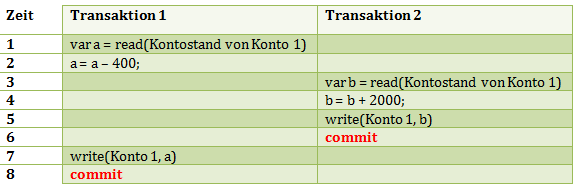
\includegraphics{res/themenkorb_5/lostupdate.png}
\end{figure}
\subsubsection{Dirty Read}
\begin{itemize}
    \item Kommt nur in Zusammenhang mit Rollback vor!
    \item Eine Transaktion liest Werte von einer anderen, welche im Nachinein wieder rückgängig (Rollback) gemacht wird!
\end{itemize}
\begin{figure}[H]
    \centering
    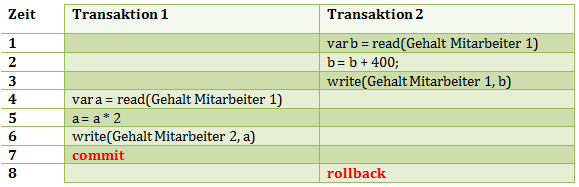
\includegraphics{res/themenkorb_5/dirtyread.png}
\end{figure}
\subsubsection{Non-Repeatable Read}
\begin{itemize}
    \item Entsteht dann, wenn lesende Vorgänge von einer anderen Transaktion unterbrochen werden!
    \item Beim nächsten Read liefert die Abfrage dann andere Ergebnisse, da hier keine 2. Transaktion "dazwischenpfuscht"!
\end{itemize}
\begin{figure}[H]
    \centering
    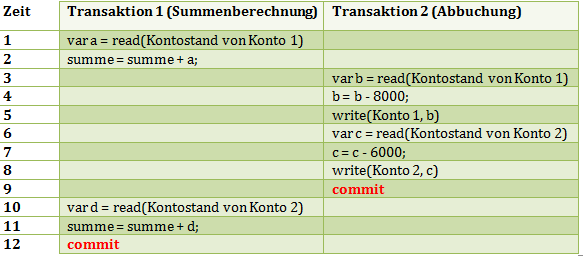
\includegraphics{res/themenkorb_5/nonrepeatableread.png}
\end{figure}
\subsubsection{Phantom}
\begin{itemize}
    \item Kommt meist im Zusammenhang mit Aggregatfunktionen vor, wenn sich z.B. durch eine andere Transaktion die Anzahl an Record ändert!
\end{itemize}
\begin{figure}[H]
    \centering
    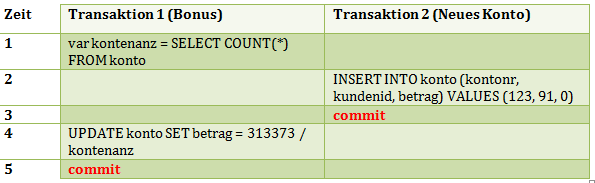
\includegraphics{res/themenkorb_5/phantom.png}
\end{figure}

\subsection{Serialisierbarkeit}
\begin{itemize}
    \item Als serialisierbar wird ein Ausführungsplan (Gibt an, welche Transaktion ausgeführt wird) dann bezeichnet, wenn das Ergebnis das selbe als jenes eines seriellen Ablaufes ist
    \item Überprüfung von Serialisierbarkeit $\implies$ Es wird ein Graph mit allen Operation aufgebaut; wenn dieser keinen Cycle enthält $\implies$ Serialisierbar (In gewisser Reihenfolge)!
\end{itemize}

\subsection{Lösungsmöglichkeiten}
\subsubsection{Sperrverfahren}
\begin{itemize}
    \item Pessimistisch
    \begin{itemize}
        \item Es wird davon ausgegangen, dass Konflikte auftreten $\implies$ Objekte werden von Anfang an gesperrt
    \end{itemize}
    \item Optimistisch
    \begin{itemize}
        \item Es wird davon ausgegangen, dass keine Probleme auftreten $\implies$ Falls doch, muss die Datenbank reagieren!
    \end{itemize}
    \item Timestamp
    \begin{itemize}
        \item Jede Transaktion enthält Startzeitpunkt $\implies$ Konflikt tritt auf, wenn jüngere Transaktion die gleichen Daten beschreibt!
    \end{itemize}
\end{itemize}
\subsubsection{Sperrebenen}
\begin{itemize}
    \item Je feiner, desto aufwändiger, aber höhere Parallelität
    \item Je gröber, desto leichter, aber geringere Parallelität
    \item Ebenen
    \begin{itemize}
        \item Datenbank
        \item Tabelle
        \item Physischer Block / Seite
        \item Zeile
    \end{itemize}
\end{itemize}
\subsubsection{Arten von Sperren}
\begin{itemize}
    \item X-Lock $\implies$ Exklusiv, Read/Write erlaubt; es können keine weiteren Locks gesetzt werden!
    \item S-Lock $\implies$ Shared, Read erlaubt; es können weitere S-Locks gesetzt werden!
\end{itemize}